\chapter{はじめに}

\section{研究背景}
本研究の背景には,ニューラルネットワークを用いた深層学習と格子ボルツマン法(Lattice Boltzmann Method, LBM)の二つの重要な要素がある.一方の深層学習は機械学習の一分野であり,複数の隠れ層を持つニューラルネットワークを使って複雑なパターンを学習する手法である\cite{doi:10.1126/science.1127647}.近年盛んに研究されていて応用先の一つに気象予測があり\cite{Schultz2021},\ref{subsec:graphcast}項や\ref{subsec:chen2021}項で述べるようにいくつかのエンコーダ-デコーダモデルが提案されている.他方で,格子ボルツマン法は1990年代以降に発展した比較的新しい数値流体力学の手法であり,個々の粒子のふるまいを扱うのではなく,格子状に分割した空間内で各格子点上の離散化された速度分布関数を解くものである\cite{doi:10.1146/annurev.fluid.30.1.329}.この手法の長所として並列計算と相性がよいことが挙げられ,GPUやTPUのようなプロセッサ上で効率的に計算することができる\cite{Satofuka1999}.これはニューラルネットワークにも共通する特性である\cite{OH20041311}.

本研究では特に気象予測のうち風速予測を取り扱う.風速予測は,風力発電の発電量を予測するために不可欠であり,また風速が強いときには風力発電機を停止させる必要があるため,この運用において重要な役割を果たす.特に山間地などの陸地の風速や風向はその地形が乱流を生むために予測しづらい傾向にあると言われており\cite{YAN2022112519},精度の良い予測モデルの開発が喫緊の課題である.

\section{先行研究 \label{sec:previous-studies}}
まず\ref{subsec:conventional-weather-forecast}項では特に気象庁やヨーロッパ中期予報センター(ECMWF)で利用されている気象予測の従来手法である,数値予報及びアンサンブル予報について述べる.続いて気象予測に深層学習を用いた研究について,それぞれ\ref{subsec:graphcast}項ではGoogle Deepmind社(2023)が発表した全球中期予報モデルGraphCastを,\ref{subsec:chen2021}項では特に本研究のタスクと計算規模に近いChenら(2021)による正方形領域での風速予測モデルを紹介する.最後に,\ref{subsec:pinns}項では気象予測モデルではないが,物理法則をニューラルネットワークに組み込むことで,データが少ない場合でも高精度な流体数値計算を行うRaissiら(2020)によるPhysics-Informed Neural Networks(PINNs)について述べる.

\subsection{数値予報及びアンサンブル予報 \label{subsec:conventional-weather-forecast}}
数値予報と呼ばれるモデルでは,大気や海洋,陸地を格子状に分割しそれぞれの格子点にある時刻の気温,風,海面温度,地面温度などの観測値を割り当て,流体力学や熱力学的な非線形偏微分方程式から導かれる計算によって逐次的に将来の状態を予測する\cite{KishochouNWP}\cite{77785}.その概要図を図\ref{fig:conventional-weather-forecast}に示す.この図からわかるように,気温や風,海面温度,地面温度,降水量,地形,植生など多くの情報が予測に用いられるため,その計算量は膨大である.例として,気象庁の全球(地球全体)モデルの数値予報では,8コアのCPUプロセッサ(IBM POWER7 3.83GHz)を160個用い,約20分間計算することで結果を得ている\cite{Aranami2016}.

しかし,一般的に非線形偏微分方程式はカオス的な性質を持つため(初期値鋭敏性)\cite{hilborn2000chaos},初期値や物理パラメータの誤差などによって数値予報の不確実性が生じる.加えて一般的に知られている方程式は近似的に自然現象を再現するものであり,大気や自然の振る舞いを完璧に記述する方程式は知られていない\cite{nwpkaisetu2023}.そこで,数値計算による決定論的予報に対して,その結果にどれほどの誤差が含まれるかを評価するためにアンサンブル予報と呼ばれる手法が用いられる\cite{nwpkaisetu2023}.アンサンブル予報では,初期値や物理パラメータに小さな摂動を与えて複数の数値予報を行う(このときの各予報をアンサンブルメンバーという).その結果を統計的に解析することで,予報の不確実性を評価することができる.図\ref{fig:ensemble-forecast}はアンサンブル予報から得られた台風進路の予報の例である\cite{nwpensemble2018}.オレンジ色の実線が各アンサンブルメンバーが異なる初期値から計算された結果を表しており,それらの範囲内に黒実線で表される実際の台風進路が収まっていることがこの図からわかる.

\begin{figure}[bp]
    \centering
    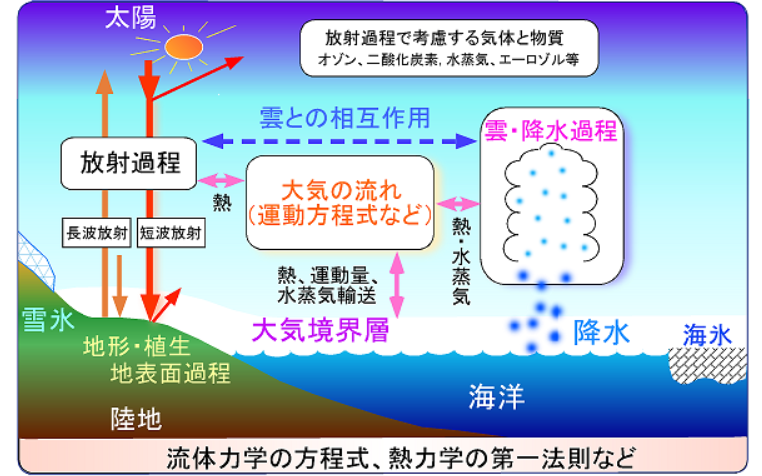
\includegraphics[width=0.8\textwidth]{./introduction/figs/numerical_weather_prediction.png.eps}
    \caption{数値予報の概要図\cite{KishochouNWP}}
    \label{fig:conventional-weather-forecast}
\end{figure}

\begin{figure}[bp]
    \centering
    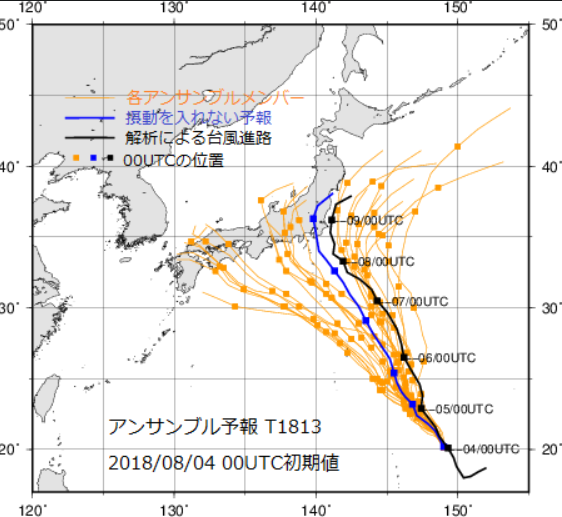
\includegraphics[width=0.7\textwidth]{./introduction/figs/ensemble.png.eps}
    \caption{アンサンブル予報から得られた台風進路の予報の例\cite{nwpensemble2018}}
    \label{fig:ensemble-forecast}
\end{figure}

\subsection{GraphCastによる気象予測 \label{subsec:graphcast}}
Google Deepmind社のLamら(2023)は,深層学習をベースにした全球中期予報モデルGraphCastを提案した\cite{Lam2023}.ここで中期予報とは,最大10日間までの予報を指している.彼らのモデルの概要図を図\ref{fig:graphcast_architecture}に示す.図\ref{fig:graphcast_architecture}(a),(b),(c)が示すようにGraphCastは,入力された時刻の気温,風速,海面温度,地面温度,降水量などの気象情報から1ステップ先の気象情報を予測しそれを繰り返すことで逐次将来の気象情報を予測をしていくモデルである.このモデルは図\ref{fig:graphcast_architecture}(d),(e),(f)が示すように,エンコーダ,プロセッサ,デコーダの3つの部分から成る.エンコーダは入力された気象情報をマルチメッシュグラフと呼ばれる構造に変換する.プロセッサではこのグラフ構造を用いて,図\ref{fig:graphcast_architecture}(g)に示すように遠近のいくつかの頂点から情報を伝達し各頂点の情報を更新する.デコーダはプロセッサの出力をグラフ構造から元の気象情報の形式に変換する.

\begin{figure}[bp]
    \centering
    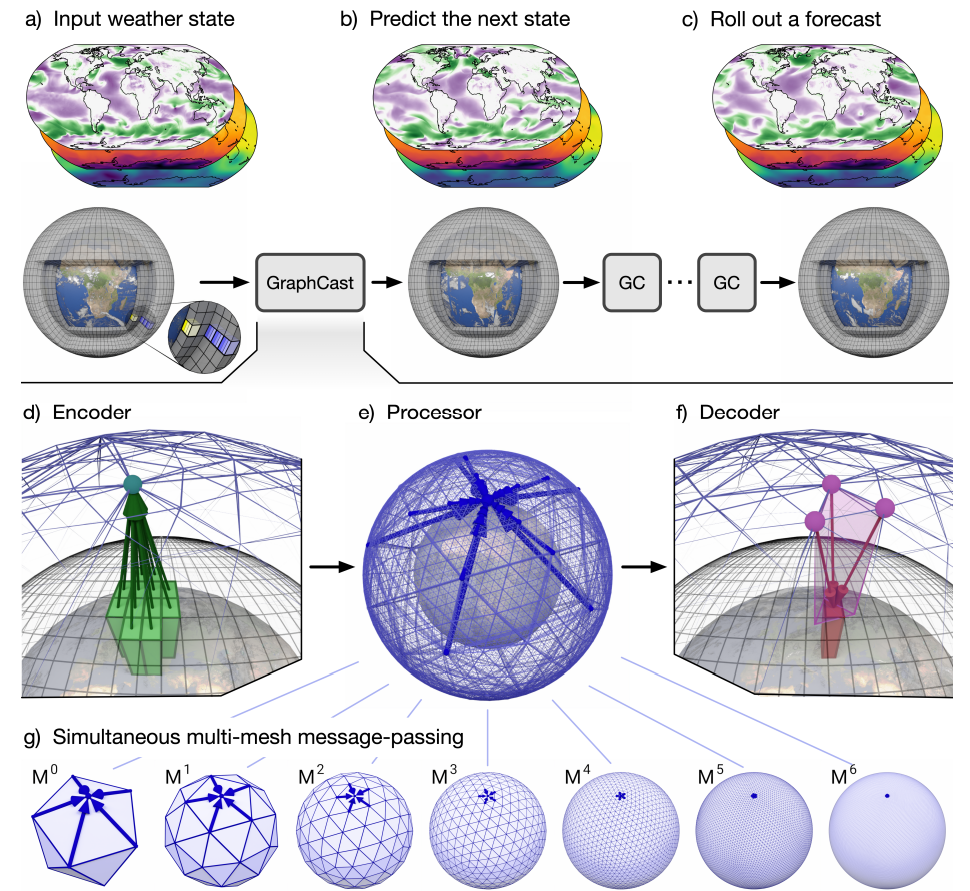
\includegraphics[width=0.9\textwidth]{./introduction/figs/graphcast-overview.png.eps}
    \caption{Lamら(2023)のモデルの概要図\cite{Lam2023} (a) 入力される気象情報 (b) 1ステップ先の予測された気象情報 (c) 数ステップ先の予測された気象情報 (d) エンコーダ (e) プロセッサ (f) デコーダ (g) マルチメッシュグラフが情報をやり取りする様子}
    \label{fig:graphcast_architecture}
\end{figure}

ECMWFで全球中期予報に用いられているHRESモデル\cite{HRES}に比べてGraphCastは$500\mathrm{hPa}$面のジオポテンシャル\cite{Geopotential}予測の二乗平均平方根誤差(Root Mean Squared Error, RMSE)が$7-14\%$低く,風速や気圧,温度などその他の多くの予測についても精度が上回った.また,図\ref{fig:cyclone_track}に示すように,特異的な気象現象であるサイクロンの軌跡予測についてもHRESモデルの精度を上回った.

彼らは,このモデルが10日分の予測をするのに単一のTPUプロセッサでも1分もかからないため,従来の手法に比べて計算量の観点においても大きいアドバンテージを有していると主張している.しかしモデルの学習には32個ものTPUプロセッサを1週間用いる必要があり,依然として計算規模が大きい.例えば日本近辺に限った局所的な予測をすることで計算量を減らそうとしても,局所的なマルチメッシュグラフを構成できないのでこの手法を適応することは難しいと推察される.

\begin{figure}[bp]
    \centering
    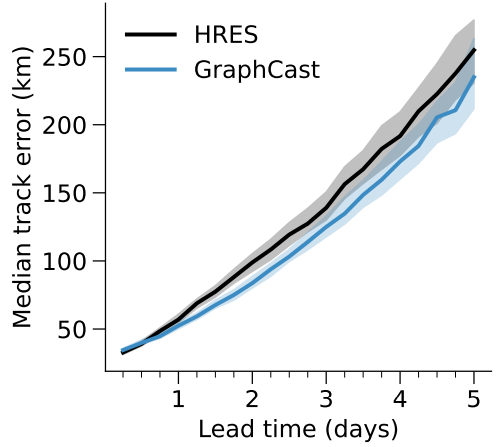
\includegraphics[width=0.4\textwidth]{./introduction/figs/cyclone_track.png.eps}
    \caption{GraphCastとHRESによるサイクロンの軌跡予測精度の比較\cite{CHEN2021114451}}
    \label{fig:cyclone_track}
\end{figure}

\subsection{CNNとLSTMを用いた正方形領域での風速予測 \label{subsec:chen2021}}
ここでは,深層学習の手法を用いて全球予測ではなく局所的な短期予測をするモデルを紹介する.Chenら(2021)は,CNN(Convolutional Neural Network)\cite{Yamashita2018}とLSTM(Long Short-Term Memory)\cite{10.1162/neco.1997.9.8.1735}を用いたモデルによる正方形領域での風速予測を行った\cite{CHEN2021114451}.彼らのモデル概要図を図\ref{fig:chen2021_architecture}に示す.この図において,エンコーダとデコーダの部分にCNNが用いられており,これにより正方形領域における格子点上の風速の空間的なパターンを学習している.また,エンコーダの出力をLSTMに入力し,更にその出力をデコーダに入力している.このLSTMのユニットにより,時間的なパターンも学習している.
\begin{figure}[bp]
    \centering
    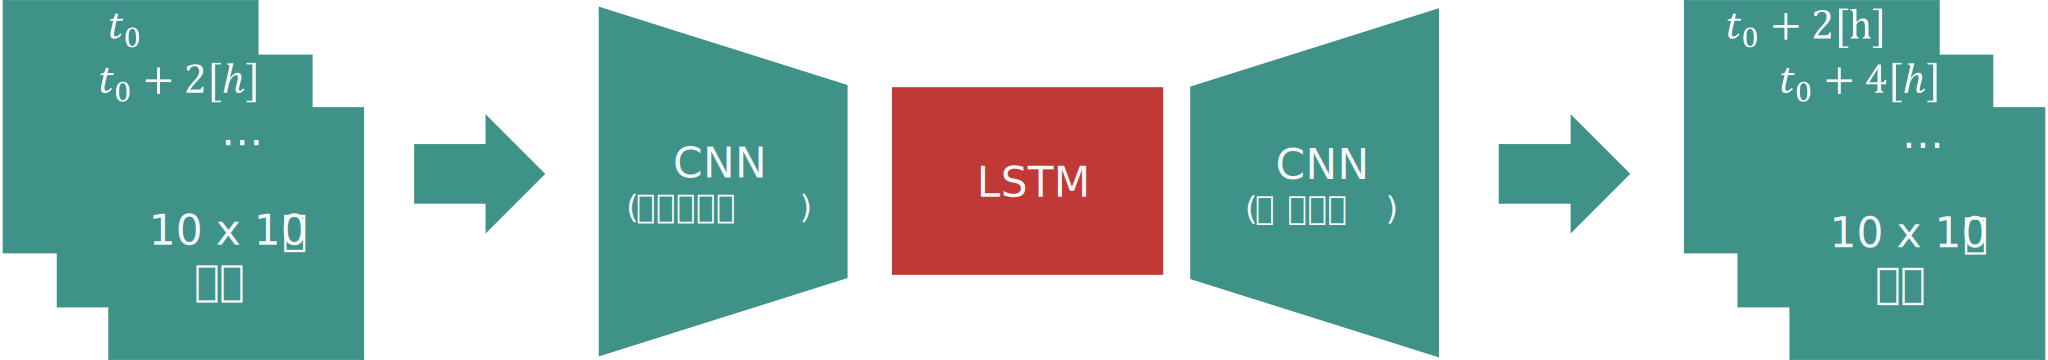
\includegraphics[width=0.9\textwidth]{./introduction/figs/chen2021_model_overview.svg.eps}
    \caption{Chenら(2021)のモデル概要図\cite{CHEN2021114451}}
    \label{fig:chen2021_architecture}
\end{figure}

このモデルを使って,彼らは図\ref{fig:chen2021_region}に示すようにアメリカのインディアナ州内部で,2km間隔の$10 \times 10$格子点上で2時間先の風速予測を行い,単にANN(Artificial Neural Network)\cite{485891}やLSTMのみを用いたモデルに比較して精度が向上することを示した.具体的には,全体の風速予測の平均絶対誤差(Mean Absolute Error, MAE)が$0.35 \mathrm{m/s}$減少し,これはPersistence モデル,ANNのみのモデル, LSTMのみのモデルの結果に比べてそれぞれ$32.7\%$, $28.8\%$, $18.9\%$低い値であると主張している.ここで,Persistence モデルとは,風速の時間変化を考慮せず,直前の風速をそのまま予測値とするモデルである.
\begin{figure}[bp]
    \centering
    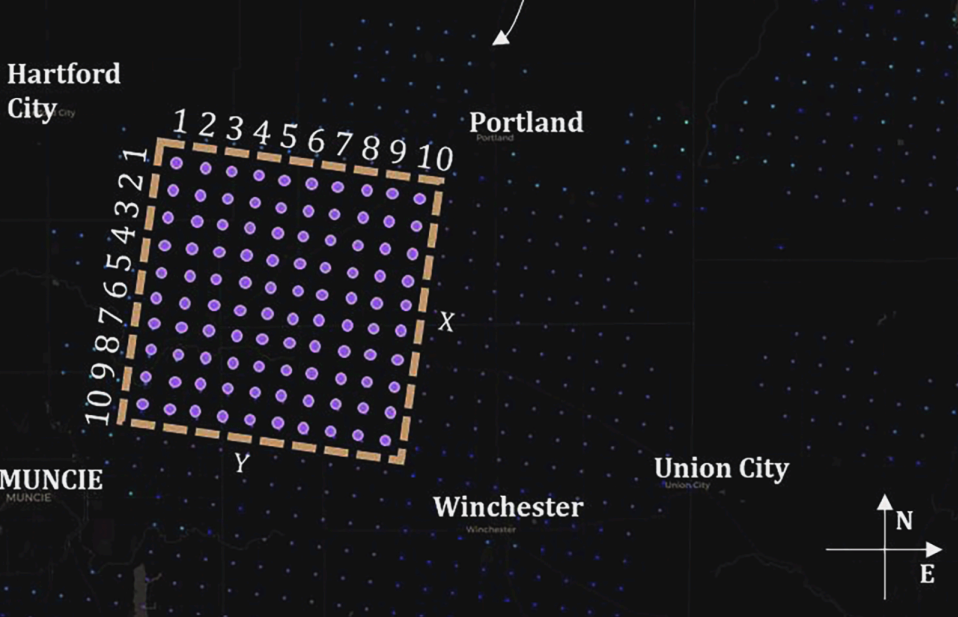
\includegraphics[width=0.8\textwidth]{./introduction/figs/chen2021_region.png.eps}
    \caption{Chenら(2021)が風速予測を行った範囲\cite{CHEN2021114451}}
    \label{fig:chen2021_region}
\end{figure}

\subsection{Physics-Informed Neural Networks \label{subsec:pinns}}
Raissi(2020)らは,物理学の知識をニューラルネットワークに組み込むことで,データが少ない場合でも高精度な予測を行うことができるPhysics-Informed Neural Networks(PINNs)というモデルを提案した\cite{PINNs2020}.このモデルは流体のシミュレーションに使われることが多く\cite{app13126892},ここでもその用途を想定する.彼らの提案したモデル概要図を図\ref{fig:pinns-overview}に示す.
\begin{figure}[bp]
    \centering
    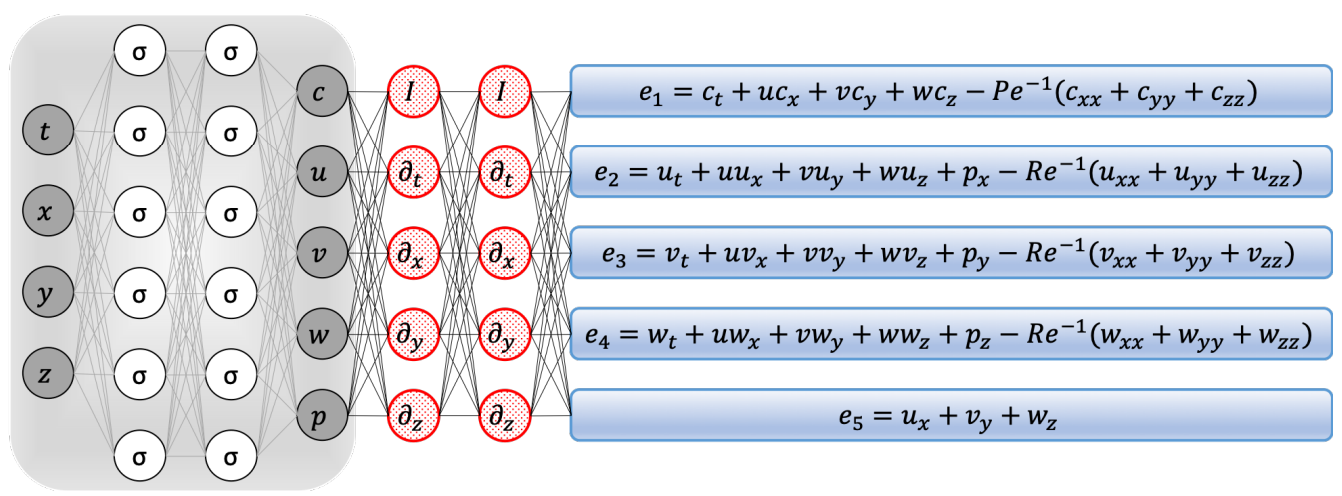
\includegraphics[width=0.9\textwidth]{./introduction/figs/PINNs_overview.png.eps}
    \caption{Raissiら(2020)のモデル概要図\cite{PINNs2020}}
    \label{fig:pinns-overview}
\end{figure}
この図が示すように,彼らのモデルは座標$x$,$y$,$z$と時刻$t$を入力とし,それに対応する流体のパッシブスカラーの濃度$c$,流体の速度$u$,$v$,$w$,そして流体の圧力$p$を出力する.なおパッシブスカラーとは,流体の流れによって変化するが流体の流れに影響を与えない物理量のことであり,例えば流体に溶けた微量な染料の濃度などが挙げられる\cite{Lesieur1990}.

彼らのモデルは,損失関数(\ref{subsection:neuron-principles}項参照)に物理的な微分方程式からどれだけモデルの出力が乖離しているかを表す項を組み込むことで,物理法則を満たすように学習をする.図\ref{fig:pinns-overview}中では$e_1$,$e_2$,$e_3$,$e_4$,$e_5$がこの項に当たる.このとき,物理量の座標微分や時間微分は,\ref{subsection:automatic-differentiation}項に述べるように自動微分を使って導くことができる.実測データが少ない場合でも,それ以外の座標と時刻を入力した場合の損失が小さくなるようにすれば,モデルの出力は物理法則に従うと彼らは主張している.

%この手法では,物理的な外力や拘束条件が既知の場合では有効であるが,例えば大気のように外力や拘束条件が不明または特定が困難な場合には損失関数をどう定めればよいのかわからず,適用するのが難しいという問題点がある. %これは良くない気がする.なぜなら,そもそもデータセットが少ない場合に適応するのが目的だから,データセットが多い場合はそもそもPINNsを使う必要がないから




\section{研究目的}
本研究では\ref{subsec:conventional-weather-forecast}項や\ref{subsec:graphcast}項で述べたような全球予測を行うモデルではなく,\ref{subsec:chen2021}項で述べたChenら(2021)の研究と同様に,日本を含む長方形領域における格子点上での短期風速予測を行うモデルを扱う.そして,ニューラルネットワークの構造にLBMを組み込むことで,それらが持つ並列計算との相性の良さを活かしつつ,流体力学の知見を用いて風速予測の精度を向上させることを目的とする.
また\ref{subsec:pinns}項で述べたRaissiら(2020)の研究とは対照的に,大気の風速予測のようにデータセットが十分あるが外力や拘束条件が不明または特定が困難な場合にも,物理法則を利用できるモデルを提案することも目的としている.

\section{論文構成}
本論文では,第\ref{section:deep-learning}節で深層学習の,第\ref{section:lbm}節で格子ボルツマン法の数理的な原理を解説し,それらを踏まえて第\ref{chap:how-to-assemble}章で提案モデルでは格子ボルツマン法をどのように深層学習モデルに組み込んだのかを解説する.第\ref{chap:experiments}章では,提案モデルの有効性を検証するため,日本近辺の風速予測を行い,従来研究のモデルと比較検討をする.